\documentclass[12pt]{article}
\usepackage[english]{babel}
\usepackage{float}
\usepackage[margin=1in]{geometry}
\usepackage{graphicx}
%\usepackage[toc,page]{appendix}
\graphicspath{ {./img/} }
\newcommand{\rpm}{\raisebox{.2ex}{$\scriptstyle\pm$}} 
\usepackage{listings}
\usepackage{xcolor}
\usepackage{indentfirst}
\usepackage{caption}
\usepackage[final]{pdfpages}


\begin{document}

\title{Joe Phaneuf \\ Computer Vision 16-720 Spring 2018 Homework 3 \\ Mar. 7, 2018 }
\date{}
\author{}
\maketitle

\newpage


%\stepcounter{section}
%%%%%%%%%%%%%%%%%%%%%%%%%%%%%%%%%%%%%%%%%%%%%%%%%%%%%%%%%%%%%%%%%%%%%%%%%%%%%%%%
%%%%%%%%%%%%%%%%%%%%%%%%%%%%%%%%%%%%%%%%%%%%%%%%%%%%%%%%%%%%%%%%%%%%%%%%%%%%%%%%
\section{Q1}
\subsection{Q1.1}
In training deep networks, a ReLU activation can be chosen over a sigmoid as it is easily differentiable, and does not suffer slow training due to saturation.

\subsection{Q1.2}
Consider a one layer network with weights $W^{1}$ , bias $b^{1}$ , input $X$ and activation function $g$. The output of this network is 
$$
out^{1} = g( W^{1} X + b^{1} )
$$
if g is a linear operator function, then there will be some modified weights and biases such that
$$
out^{1} = \hat{W}^{1} X + \hat{b}^{1}
$$

For a subsequent layer, the pre-activation is
$$
W^{2} ( \hat{W}^{1} X + \hat{b}^{1} ) + b^{2}
$$
Which, due to the properties of matrix multiplication, can be reduced to some modified weights and biases
$$
\hat { W^{2} } X + \hat { b} ^{2}
$$

$\hat { W^{2} }$ and $\hat { b} ^{2}$ are of the same dimension as $W^{1}$ and $b^{1}$, meaning no additional discriminatory information can be encapsulated by the second layer. 

A non-linear activation function makes it impossible to combine weights as demonstrated above, meaning each additional layer does add to the discriminatory power of the network.

\section{Q2}
\subsection{Q2.1.1}
Weight initialization is an important factor for training neural networks. Naively initializing weights to zero results in zero valued gradients, which prevents weight updates. Initializing with all equal weights also reduces the same gradients for each weight, so training does not function properly. 

\subsection{Q2.1.3}
I chose to initialize weights from a uniform distribution ranging from -0.1 to 0.1. This was mostly from research and some experimention. Weights that are too large can create issues by way of massive gradients, weights that are too small can take a long time to train due to very small gradients.


\subsection{Q2.4.1}
Stochastic gradient descent is more robust to non-convex error manifolds , but may take longer to reach minima. Batch gradient descent will typically converge faster given error manifolds that are reasonably convex , but can be more expensive in terms of required RAM.

\subsection{Q3.1.1}
Figure \ref{fig:accloss} shows the training and validation accuracy and loss while training on the nmist26 dataset.
\begin{figure}[H]
\centering
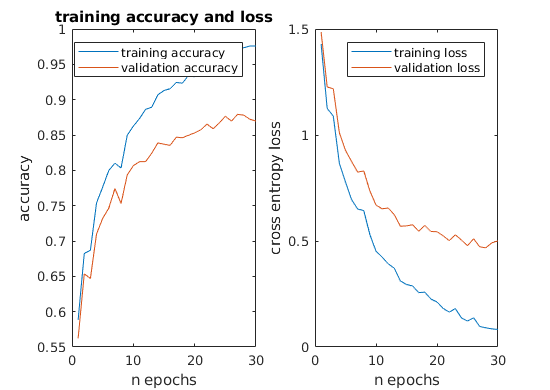
\includegraphics[page=1,width=0.4\textwidth]{q311}
\caption{Training and validation accuracy and loss} 
\label{fig:accloss}
\end{figure}   
\end{document}
